\documentclass{article}
\usepackage[margin=0.7in]{geometry}
\usepackage{amsmath}
\usepackage{amssymb}
\usepackage{bookmark}
\usepackage{graphicx}
\usepackage{float}

\title{Report for Assignment - 1: CS6370 - \\Information Retrieval}
\author{
Harsh Agarwal\\\texttt{CS15BTECH11019}
\and
Sukrut Rao\\\texttt{CS15BTECH11036}
\and
Vishwak Srinivasan\\\texttt{CS15BTECH11043}
}
\date{}

\begin{document}
\maketitle

\section{Introduction}
\begin{flushleft}
This assignment focused on empirically verifying \textbf{Zipf's Law} and \textbf{Heaps' Law} for two different datasets. Task 1 focused on the verification of the former, while Task 2 focused on the verification of the latter. Task 1 was a bit more involved than Task 2, because of the more text processing that had to be done to satisfy requirements.
\(\newline\)

Some statistics of the datasets: the first dataset (i.e., the dataset in CSV format) contains 32578 documents and the second dataset (i.e., the dataset in JSON format) contains 32912 documents.

\subsection{Pre-processing the datasets}
The main scripts provided work fine on datasets in the CSV format. For this we had to convert the dataset in JSON to CSV format. During this process we found certain parsing errors due to escape characters. These were found in lines \{9045, 9838, 13550, 14553, 16890\}, and were manually fixed by \texttt{grep}-ing and replacing the erroneous characters.
\end{flushleft}

\section{Task 1: Verification of Zipf's Law}
\subsection{Text processing of the datasets}
\begin{flushleft}
Below are the steps for processing:
\begin{enumerate}
\item Case Folding - convert all documents to lower case. For example: ``I didn't create Atlantis'' becomes ``i didn't create atlantis''.
\item Removal of special characters and digits - all special characters (quotes, commas, apostrophes, fullstops, etc.) and digits (0 to 9) were removed. This meant that at the end of this step we had nothing but raw text composed of alphabets alone. For example: ``don't'' becomes ``dont'' and ``ariane-5'' becomes ``ariane''.
\item Removal of stop words - using \texttt{NLTK}'s corpus of stop words, this was easy.
\item Stemming - using \texttt{NLTK}'s \texttt{PorterStemmer} we were able to do this.
\item Lemmatization - for this we used \texttt{NLTK}'s \texttt{WordNetLemmatizer}.
\end{enumerate}

For the base analysis, points 1 and 2 are considered. Subsequent processing involves steps 3 through 5.
\end{flushleft}
\newpage

\subsection{Plots, Top 20 words and Observations}
\subsubsection{Plots}
\begin{flushleft}
Below are the plots obtained for Dataset 1 (CSV) and Dataset 2 (JSON).
\begin{figure}[H]
\begin{minipage}{0.45\linewidth}
\centering
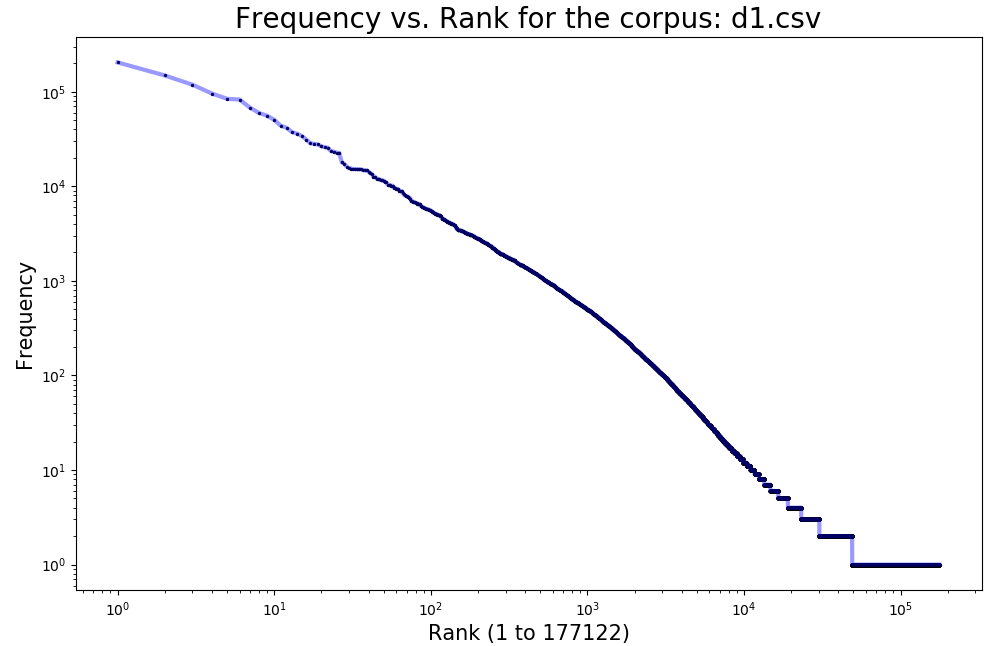
\includegraphics[width=0.75\textwidth]{./images/dataset-1-t1-0.png}
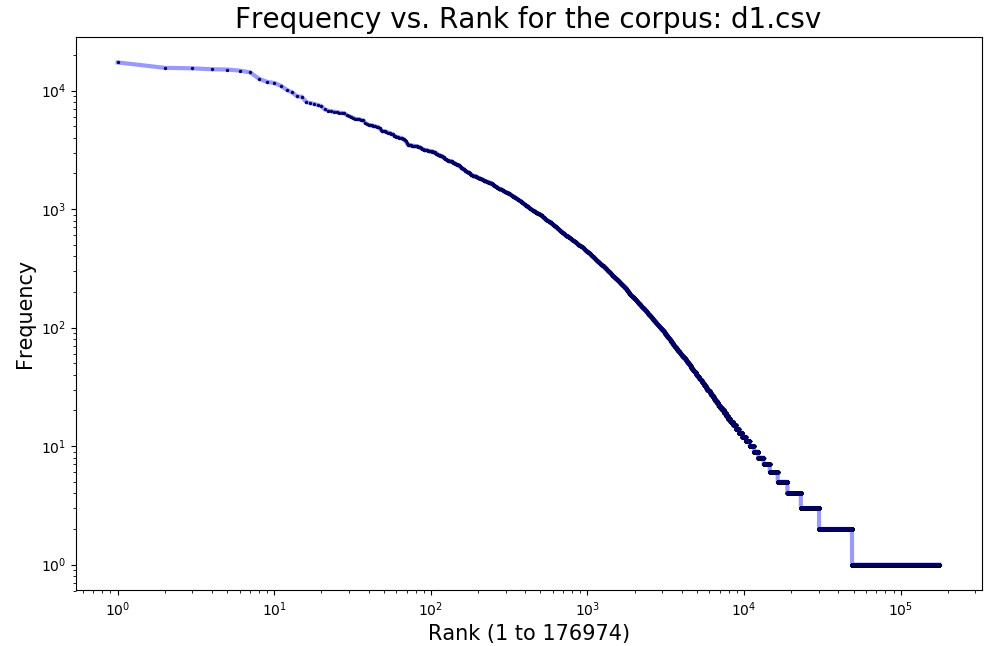
\includegraphics[width=0.75\textwidth]{./images/dataset-1-t1-1.png}
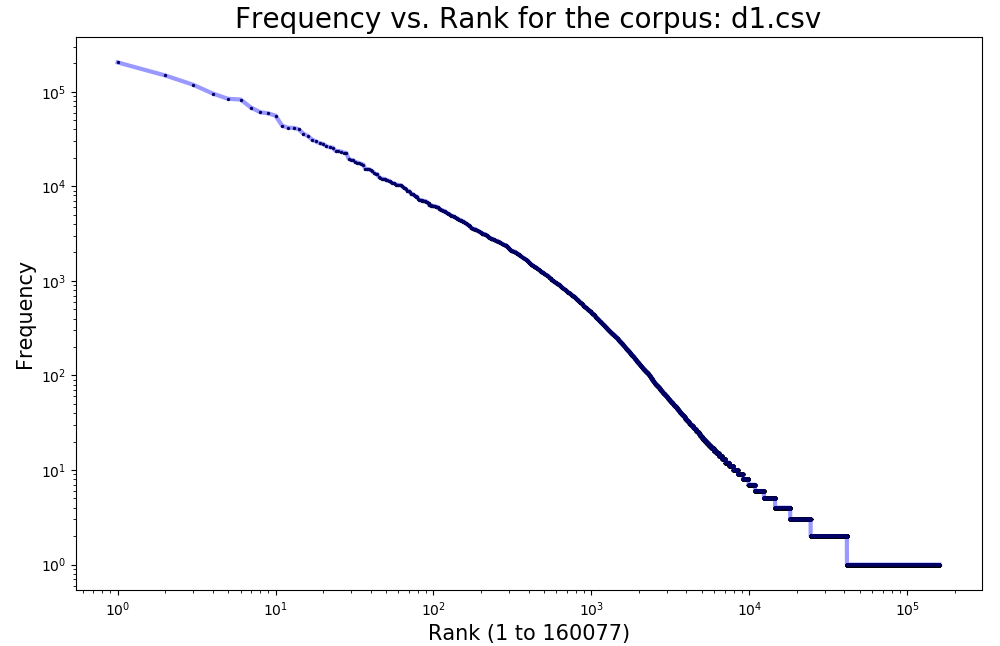
\includegraphics[width=0.75\textwidth]{./images/dataset-1-t1-2.png}
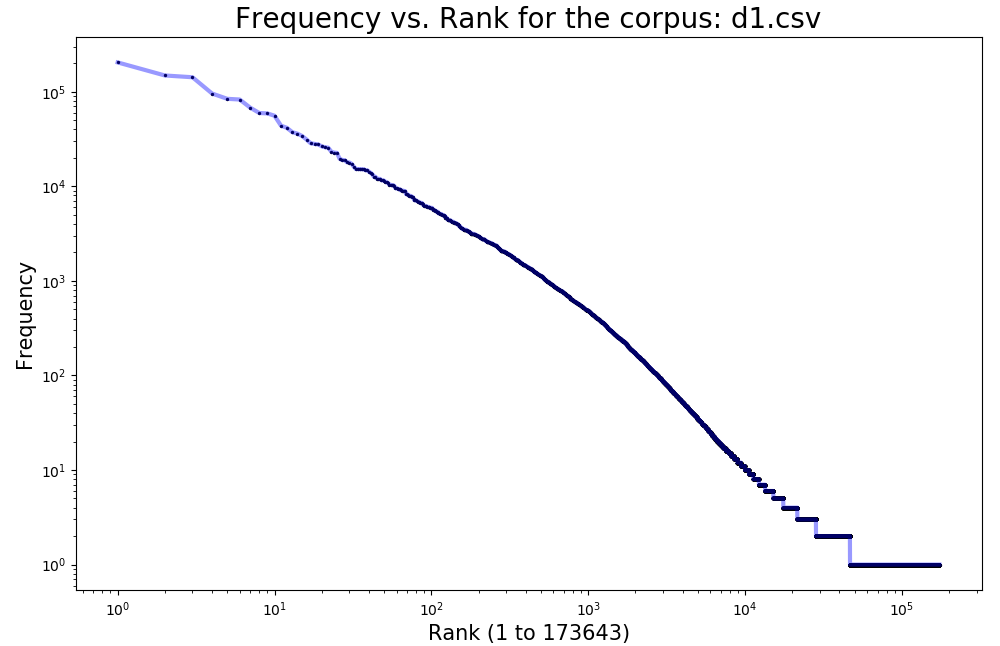
\includegraphics[width=0.75\textwidth]{./images/dataset-1-t1-3.png}
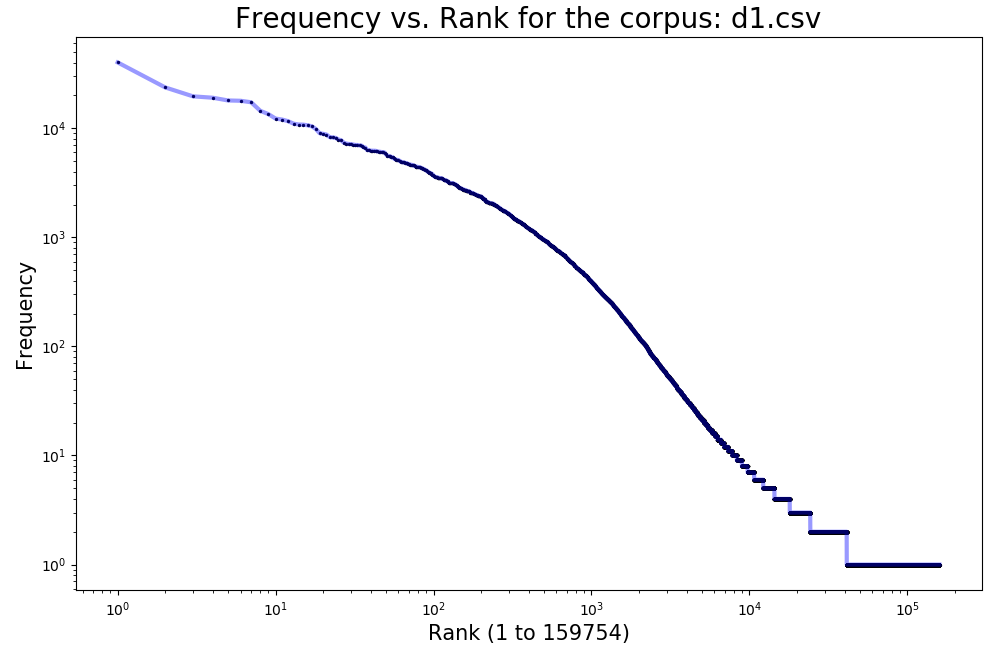
\includegraphics[width=0.75\textwidth]{./images/dataset-1-t1-4.png}
\end{minipage}
\hfill
\begin{minipage}{0.45\linewidth}
\centering
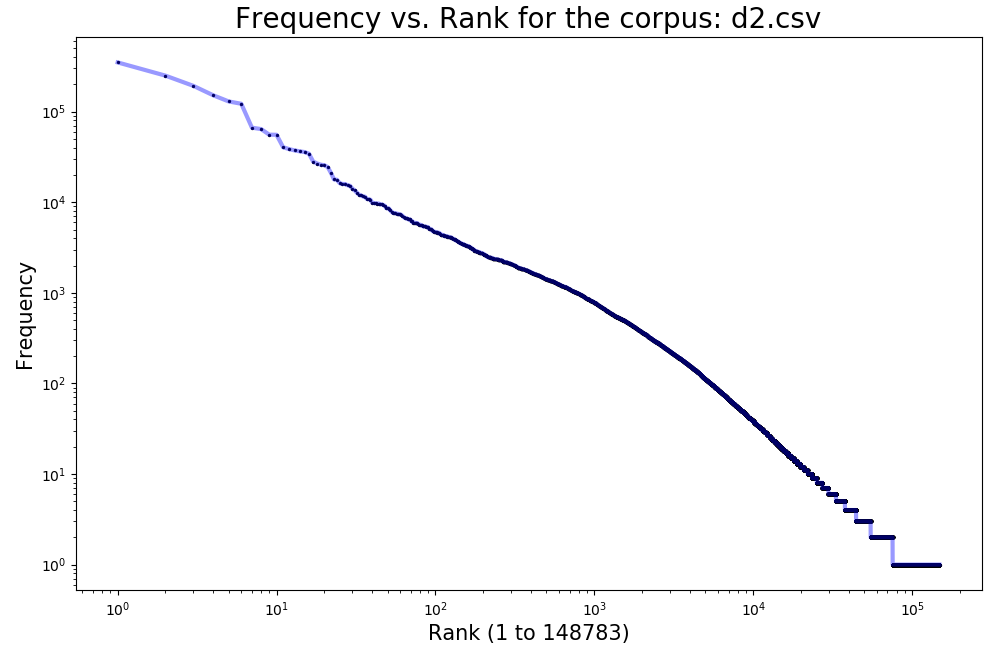
\includegraphics[width=0.75\textwidth]{./images/dataset-2-t1-0.png}
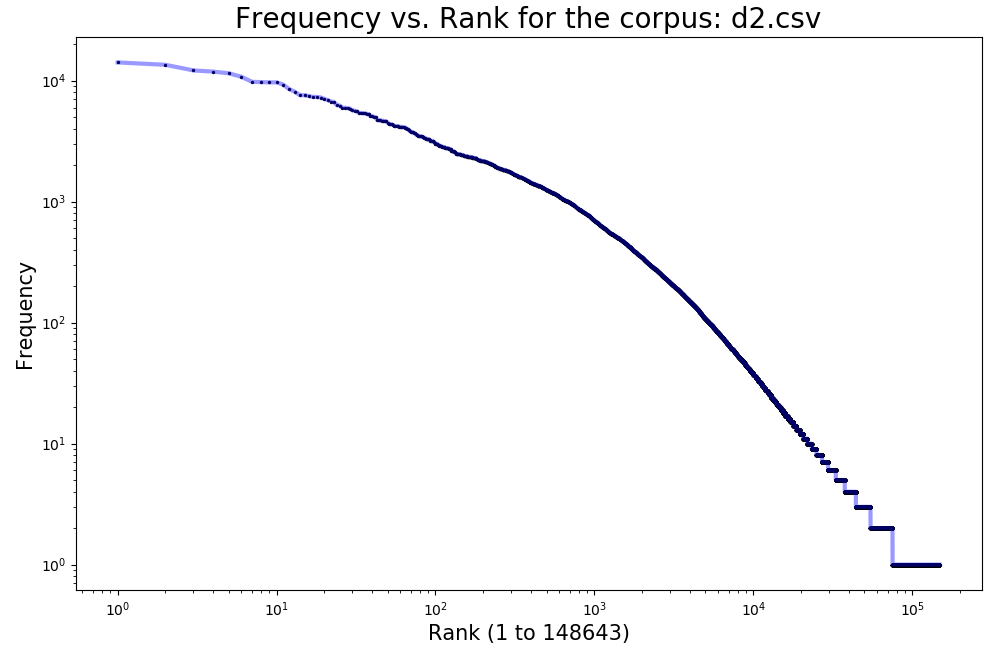
\includegraphics[width=0.75\textwidth]{./images/dataset-2-t1-1.png}
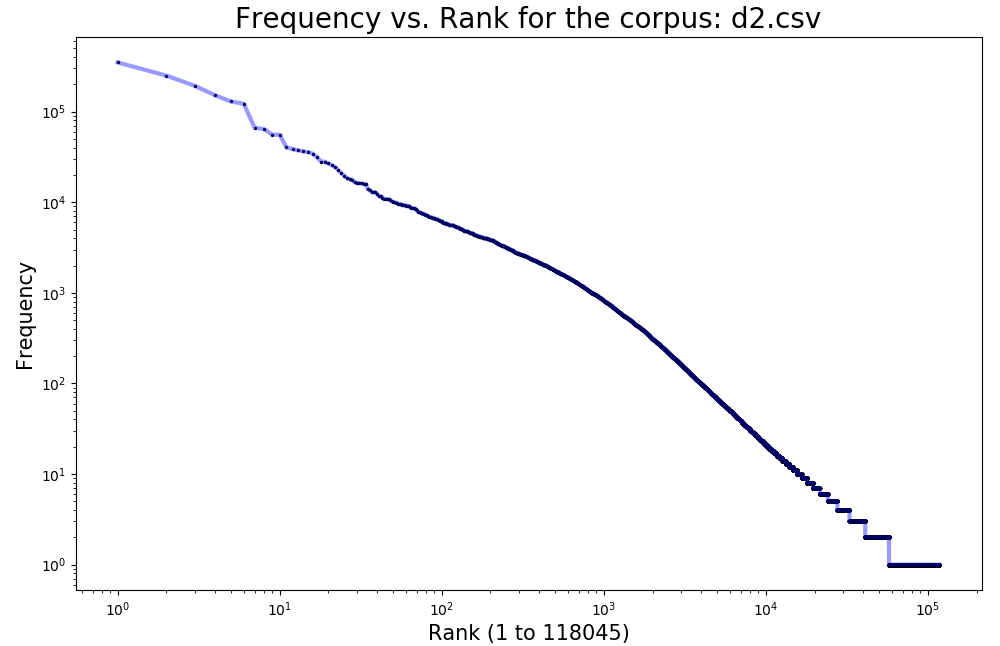
\includegraphics[width=0.75\textwidth]{./images/dataset-2-t1-2.png}
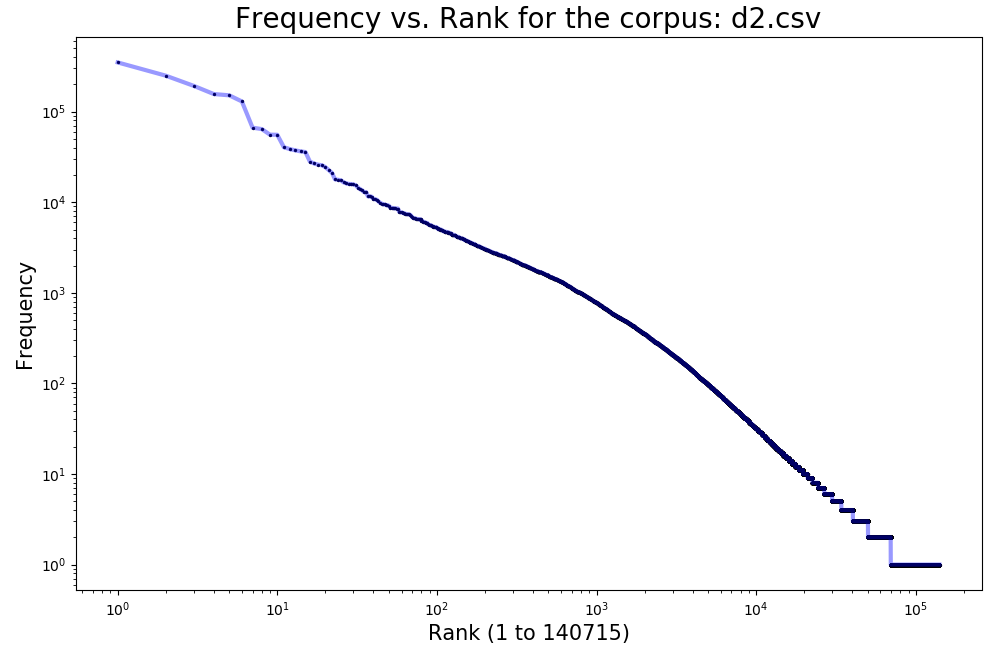
\includegraphics[width=0.75\textwidth]{./images/dataset-2-t1-3.png}
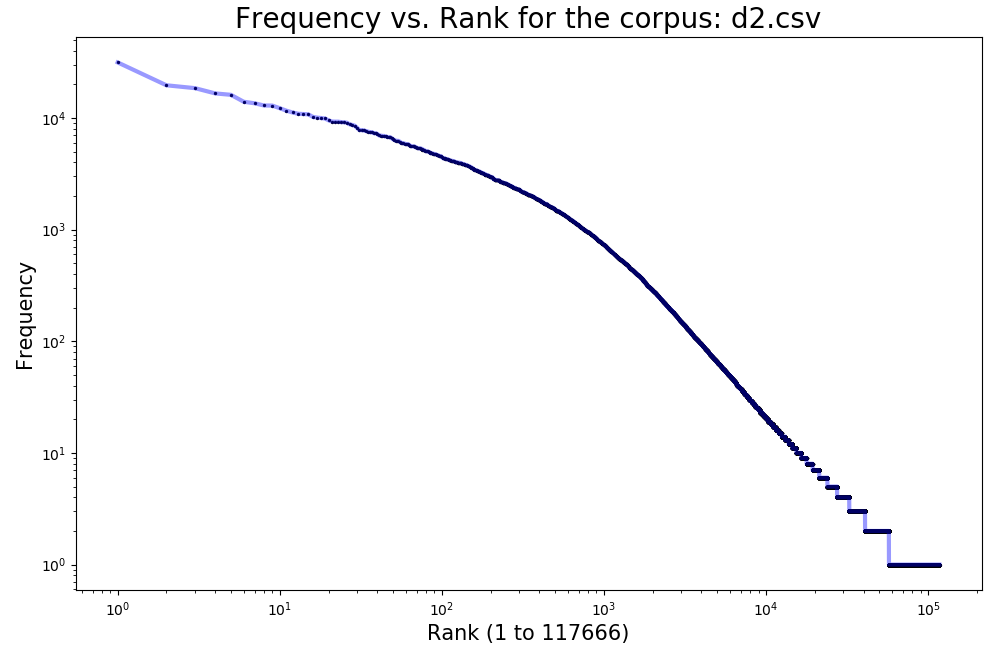
\includegraphics[width=0.75\textwidth]{./images/dataset-2-t1-4.png}
\end{minipage}
\caption{Results for Dataset 1 (Left) and Dataset 2 (Right).\newline{}These are log plots for better visualization. Each plot from top to bottom represents a sequence of processing steps.\newline{}These are (ordered from top to bottom): [1, 2], [1, 2, 3], [1, 2, 4], [1, 2, 5], [1, 2, 3, 4, 5]}
\end{figure}
\end{flushleft}

\subsubsection{Top 20 words}
\begin{flushleft}
The top 20 words obtained after each of the five sequences of processing steps are tabulated below (Dataset 1 on the left, Dataset 2 on the right). Frequencies are specified in the brackets next to each word.
\begin{center}
\begin{tabular}{|p{0.08\textwidth}|p{0.37\textwidth}||p{0.08\textwidth}|p{0.37\textwidth}|}
\hline
Processing Steps & Top 20 Words & Processing Steps & Top 20 Words \\
\hline
\hline
[1,2] & the(204366), to(148692), a(118804), i(95778), is(84217), and(82792), of(67924), that(59615), in(55797), it(50473), for(43818), this(41526), be(37341), on(36058), my(34051), with(31263), can(28523), not(28099), have(27721), or(26475) &
[1,2] & the(349582), of(249661), and(192456), in(151426), to(129629), a(122159), is(66532), for(64191), with(55686), that(55531), this(40477), we(38588), on(37331), by(36459), are(35817), as(34330), was(28140), an(26757), be(25963), were(25632)\\
\hline
[1,2,3] & would(17312), key(15577), server(15433), using(15154), password(15077), use(14767), security(14275), like(12590), user(11851), im(11610), data(11005), one(10183), know(9672), access(8941), could(8887), way(8017), get(7848), secure(7724), file(7555), used(7407) &
[1,2,3] & results(14161), data(13526), study(12158), patients(11881), using(11515), also(10779), model(9790), system(9733), used(9683), paper(9674), two(9288), may(8521), one(8114), use(7593), p(7578), analysis(7464), time(7347), different(7332), based(7260), information(7069)\\
\hline
[1,2,4] & the(204366), to(148717), a(118804), i(95783), is(84217), and(82794), of(67924), that(60797), it(59041), in(55805), for(43818), be(41565), thi(41527), use(40149), on(36061), my(34051), with(31268), have(29873), can(28526), not(28099) &
[1,2,4] & the(349584), of(249661), and(192462), in(151454), to(129631), a(122215), is(66532), for(64196), with(55686), that(55551), thi(40479), we(38588), on(37345), by(36459), are(35822), as(34330), use(31440), wa(28147), be(28021), an(26780)\\
\hline
[1,2,5] & the(204366), to(148692), a(142398), i(95783), is(84217), and(82792), of(67924), that(59615), it(59042), in(55805), for(43818), this(41526), be(37349), on(36058), my(34051), with(31263), can(28523), not(28099), have(27721), or(26478) &
[1,2,5] & the(349582), of(249661), and(192456), a(156489), in(151454), to(129629), is(66532), for(64191), with(55686), that(55531), this(40477), we(38588), on(37331), by(36459), are(35821), wa(28147), an(26780), be(25969), were(25632), from(24417)\\
\hline
[1,2,3,4,5] & use(40149), secur(23682), password(19616), key(19046), server(17984), user(17868), would(17312), encrypt(14454), like(13477), attack(12268), file(12010), im(11612), data(11021), one(10826), know(10786), access(10644), get(10408), certif(9827), way(9003), could(8888) &
[1,2,3,4,5] & use(31440), studi(19617), result(18490), model(16591), system(16111), patient(13965), data(13536), method(12932), effect(12907), differ(12233), cell(11615), present(11196), develop(10902), show(10831), also(10779), paper(10230), function(10075), activ(9980), increas(9893), perform(9526)\\
\hline
\end{tabular}
\end{center}
\end{flushleft}

\subsubsection{Observations}
\begin{flushleft}
Statistically, a few things worth noting:
\begin{itemize}
\item The number of terms before stopword removal is greater than the number of terms after stopwords have been removed.
\item The number of terms before stemming / lemmatization is greater than the number of terms after stemming / lemmatization has been performed.
\item The number of terms after stemming is smaller than the number of terms after lemmatization.
\item The number of terms after performing stopword removal, stemming and lemmatization is smallest amongst all processing steps performed.
\end{itemize}
From the above points, one can build an ordering the processing steps based on the number of terms obtained:
\begin{center}
Terms from raw data \(>\) Terms from stopword removal \(>\) Terms from lemmatization \(>\) Terms from stemming \(>\) Terms from stopword removal, lemmatization and stemming
\end{center}

From the plots, note that these are log-log plots of the rank versus frequency. Using a generalized power law i.e.,
\begin{equation}
\label{gen-zipf}
y = \frac{c}{x^{m}} \Rightarrow \log y = \log c - m \log x
\end{equation}
we found out the best parameters. Ideally we would like for \(m\) to be as close to \(1\) as possible. Below are the values found for the two datasets, after each processing:
\begin{center}
\begin{tabular}{|c|c|c|c|c|c|}
\hline
\multicolumn{3}{|c|}{Dataset 1} & \multicolumn{3}{|c|}{Dataset 2}\\
\hline
Processing & \(m\) & Intercept (\(\log c\)) & Processing & \(m\) & Intercept (\(\log c\))\\
\hline
\hline
[1,2] & 1.018 & 5.109 & [1,2] & 1.424 & 7.183\\
\hline
[1,2,3] & 0.998 & 5.011 & [1,2,3] & 1.407 & 7.099\\
\hline
[1,2,4] & 0.943 & 4.684 & [1,2,4] & 1.406 & 6.932\\
\hline
[1,2,5] & 0.987 & 4.942 & [1,2,5] & 1.408 & 7.06\\
\hline
[1,2,3,4,5] & 0.922 & 4.581 & [1,2,3,4,5] & 1.386 & 6.833\\
\hline
\end{tabular}
\end{center}

In both the datasets, we are able to see that more processing causing the slope to decrease in Eqn \ref{gen-zipf}. The intercept is affected in a similar manner. From a raw graphical perspective, we can notice that the raw data is more linear than the ones obtained after processing. In fact, the linearity fades as we perform more processing on the dataset in the form of stopword removal and/or stemming and/or lemmatization.
\end{flushleft}

\section{Task 2: Verification of Heaps' Law}
Text processing for this task involved steps 1 and 2 describes in the previous section.
\subsection{Plots and Observations}
\subsubsection{Plots}
\begin{flushleft}
\begin{figure}[H]
\begin{minipage}{0.45\linewidth}
\centering
\includegraphics[width=0.75\textwidth]{./images/dataset-1-t2-0.png}
\end{minipage}
\hfill
\begin{minipage}{0.45\linewidth}
\centering
\includegraphics[width=0.75\textwidth]{./images/dataset-2-t2-0.png}
\end{minipage}
\caption{Results for Dataset 1 (Left) and Dataset 2 (Right).\newline{}These are log plots for better visualization.}
\end{figure}
\end{flushleft}

\subsubsection{Observations}
\begin{flushleft}
Visual observation suggests that these plots are very ``linear''. This verifies the generalized Heaps' Law. Fitting the log-log plot to a linear function, gives us the values of the constants in Heaps' Law:
\begin{equation}
V = \alpha T^{\beta} \Rightarrow \log V = \beta \log T + \log \alpha
\end{equation}
Below are the computed values of \(\beta\) and \(\log \alpha\) from a best linear fit:
\begin{center}
\begin{tabular}{|c|c|c|c|}
\hline
\multicolumn{2}{|c|}{Dataset 1} & \multicolumn{2}{|c|}{Dataset 2}\\
\hline
\(\beta\) & \(\log \alpha\) & \(\beta\) & \(\log \alpha\)\\
\hline
\hline
0.731 & 0.379 & 0.606 & 1.07 \\
\hline
\end{tabular}
\end{center}

From Wikipedia, for typical English text corpora, the values of \(\beta\) is between 0.4 and 0.6, while the values of \(\alpha\) is between 10 and 100, which means \(\log \alpha\) is between 1 and 2. From this, one can call dataset 1 as a ``non-typical'' English text corpus, while dataset 2 is still close to the ranges.
\(\newline\)

On close observation, one can see that there are more points concentrated at the left end of the seemingly straight line. This is nothing very special, it is primarily due to the nature of the log-log plot.
\end{flushleft}
\end{document}
